
\section{Iterative Methods for Neutron Transport}
Solving the transport equation involves several nested iterative solvers. To discuss these iterative methods it is useful to think of the transport equation in operator form. 
\begin{equation}
    \bf{L}\psi = \bf{S}\psi + \bf{Q}
\end{equation}
where $\bf{L}$ is the matrix formed by discretizing the left-hand side, $[\hat{\Omega} \cdot \nabla + \Sigma(\vec{r}, E)]\psi(\vec{r}, \hat{\Omega}, E)$, using finite elements or any other discretization method and $\bf{S}\psi$ and $\bf{Q}$ are matrices representing the source terms. 

\subsubsection{Linear Solver}
The inner-most layer of iteration is the linear solve in which we treat the transport equation as a system of linear equations and solve for a vector, $\psi$, which represents the flux at several points in space. In order to do so, it must take the form ${\bf A} x = b$ where $b$ is a constant vector, but we see in this case our $b = {\bf S} \psi + {\bf Q}$ which is dependent on $\psi$ in the scattering source. To remedy this we choose $\psi$ on the right hand side to be a constant. The method by which we choose this constant, called source iteration, is the next level of iteration, detailed below. Now that $b$ is a constant vector, we are able to perform a linear solve. Solving $\textbf{A}x = b$ is well studied problem, and there are many iterative methods to choose from. Most have already been implemented in forms optimized for performance in various linear algebra libraries such as LAPACK.

\subsubsection{``Inner" Iterations}
The inner iterations solve the space-angle component for each energy group. As was mentioned above, the scattering term on the right hand side of the transport equation (\ref{eq:transport}) depends on the angular flux, $\psi$. The inner iterations, iterate on a guess of that angular flux so that it can be treated as a constant for the linear solves. The traditional method is called source iteration, which is explained in more detail below. A more advanced alternative to source iteration that is starting to gain popularity is a Krylov solver. 

\subsubsection{Multigroup or ``Outer Iterations"}
The multigroup iterations solve the energy component. When we have more than one energy group, we solve each group independently, performing source iteration on each one. In doing so, we must include the scattering from all other energy groups to the current group multiplied by the flux of the other groups. When there is no ``upscattering", meaning there is no scattering from a lower energy group to a higher energy group, we can solve each group sequentially, starting with the highest energy group, without any problems. No other groups scatter to group one, the highest energy group, the next group is only dependent on the flux from group one, which we just solved for, and so on. In the case of upscattering, an outer layer of iteration is added to converge the scattering source. The most common multigroup solver is called the Gauss-Seidel method. Other alternatives include Jacobi or multigroup Krylov. 

The three formulations that are discussed, NDA, TG-NDA, and SAAF can be solved using any combination of the solvers listed above. We will explain in detail the solvers that were used in our implementation. 

\section{Implemented Solvers}
\subsection{Linear Solver}
For our linear solver we used SciPy's conjugate gradient solver \cite{SciPy} \cite{Shewchuck1994}. CG solves the system Ax = b assuming A is a real, symmetric, positive-definite matrix. By using the finite element method, we are guaranteed that our matrix A satisfies those constraints, so CG is an applicable method for our problem.

\subsection{Within Group Solver - Source Iteration}
The inner solves are handled by a procedure known as source iteration. The $\psi$ on the right hand side of the equation starts with an initial guess. At each iteration, the linear system is solved and $\psi$ is updated with the result of that solve. This continues until the values converge. 
\begin{algorithm}
\caption{Source Iteration}
\begin{algorithmic}
\While{$res > tol$} \Comment {Iteration Index $k$}
    \State \textbf{Set up} FEM discretization of Eq.
    \State ${\bf S} \psi \gets \sigma_s \phi^{k-1}$ \Comment {Assumes one group, see multigroup below.}
    \State \textbf{Solve} system $\textbf{L}\psi= {\bf S}\psi + {\bf Q}$
    \State $res \gets max(|\psi^{k} - \psi^{k-1}|)$
\EndWhile
\end{algorithmic}
\end{algorithm}

\subsection{Multigroup Solver - Gauss Seidel}
When dealing with a multigroup problem, the scattering source is dependent not only on the flux from the current group, but from other groups as well. In the case that there is no upscattering, meaning that the flux from a lower energy group does not contribute to any higher energy group, we can solve sequentially, starting with the highest energy group and using the fluxes as we calculate them. In the case of upscattering, we must choose an initial guess for the fluxes of lower energy groups and then iterate until we find a convergent value. We use a method inspired by the Gauss-Seidel method for linear equations. When iterating, we use the flux calculated in this iteration for the higher energy groups and the flux calculated in the previous iteration for the lower energy groups. The pseudocode of the algorithm is given below. 
\begin{algorithm}
\caption{Outer Iterations: Gauss Seidel}
\begin{algorithmic}
    \While {$res > tol$} \Comment {Iteration Index $l$}
        \For {$ g \in G$}
            \State \textbf{calculate} scattering source: \State $ {\bf S} \psi = \sigma_{gg}\phi_g^{l+1} + \sum\limits_{g'=1}^{g-1} \sigma_{gg'} \phi_{g'}^{l+1} + \sum\limits_{g'=g+1}^G \sigma_{gg'}\phi_{g'}^l$
            \Procedure {Source Iteration on group $g$}{} 
        \EndProcedure
        \EndFor
        \State $res \gets max(|\phi^{l} - \phi^{l-1}|)$  \Comment {Check if sol. for each group has converged}
        \EndWhile
    \Return $\phi$
\end{algorithmic}
\end{algorithm}

\subsection{TG-NDA}
TG-NDA acclerates convergence by applying a correction at two different layers of iteration. NDA applies a correction using the drift vector at each source iteration. Two-Grid provides a correction at each Gauss-Seidel iteration. The full scheme as implemented is illustrated below with the correction terms highlighted in blue. 


\begin{figure}[H]
    \centering
    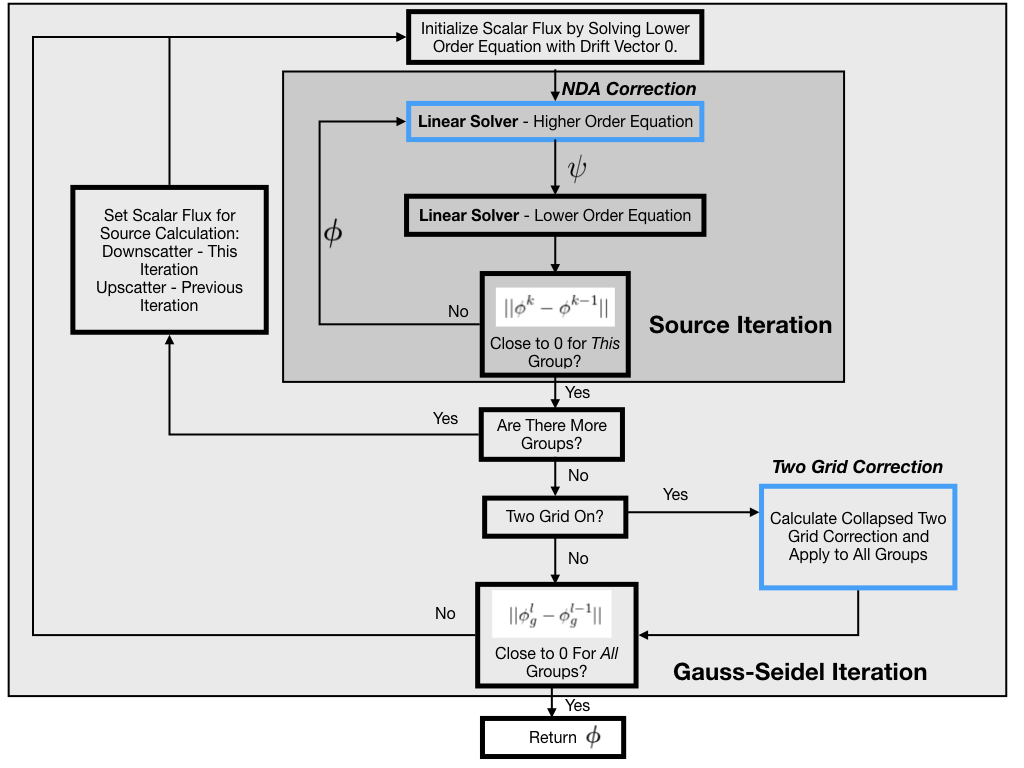
\includegraphics[width=\textwidth]{fig/TGNDAchart.png}
    \caption{Full Iterative TG-NDA Scheme}
    \label{fig:tgnda-graph}
\end{figure}